\appendix

\section{Cultural Dimension Comparison: Germany and Japan}
\label{sec:appendix-country-comparison-tool-descriptions}

The following paragraphs are excerpts from the Country Comparison tool, visualized in \cref{fig:country-comparison}.

\begin{enumerate}
%     \item \ac{pdi}
%     \begin{itemize}
%         \item \textbf{Germany}
%         Highly decentralised and supported by a strong middle class, Germany is not surprisingly among the lower power distant countries (score 35).
%         Co-determination rights are comparatively extensive and have to be taken into account by the management.
%         A direct and participative communication and meeting style is common, control is disliked and leadership is challenged to show expertise and best accepted when it's based on it.
% % old dependency versions in Japan
%         \item \textbf{Japan}
%         At an intermediate score of 54, Japan is a borderline hierarchical society.
%         Yes, Japanese are always conscious of their hierarchical position in any social setting and act accordingly.
%         However, it is not as hierarchical as most of the other Asian cultures.
%         Some foreigners experience Japan as extremely hierarchical because of their business experience of painstakingly slow decision making process: all the decisions must be confirmed by each hierarchical layer and finally by the top management in Tokyo.
%         Paradoxically, the exact example of their slow decision making process shows that in Japanese society there is no one top guy who can take decision like in more hierarchical societies.
%         Another example of not so high Power Distance is that Japan has always been a meritocratic society.
%         There is a strong notion in the Japanese education system that everybody is born equal and anyone can get ahead and become anything if he (yes, it is still he) works hard enough.
%     \end{itemize}

    \item \ac{idv}
    \begin{itemize}
        \item \textbf{Germany}
        The German society is a truly Individualist one (79).
        Small families with a focus on the parent-children relationship rather than aunts and uncles are most common.
        There is a strong belief in the ideal of self-actualization.
        Loyalty is based on personal preferences for people as well as a sense of duty and responsibility.
        This is defined by the contract between the employer and the employee.
        Communication is among the most direct in the world following the ideal to be “honest, even if it hurts” – and by this giving the counterpart a fair chance to learn from mistakes.

        \item \textbf{Japan}
        Japan scores 62 on the Individualism dimension.
        Japanese society shows the characteristics of an individualistic society.
        Japanese society does not have an extended family system like China and Korea.
        Japan has been a paternalistic society and the family name and asset was inherited from the father to the eldest son.
        The younger siblings had to leave home and make their living with their core families.
        Japanese are famous for their loyalty to their companies, which people have chosen for themselves, which is an Individualist thing to do.
        You could say that the Japanese in-group is situational.
        Japanese are more private and reserved than most other Asians.
    \end{itemize}

    \item \ac{mas}
    \begin{itemize}
        \item \textbf{Germany}
        With a score of 66 Germany is considered a Decisive society.
        Performance is highly valued and early required as the school system separates children into different types of schools at the age of ten.
        People rather “live in order to work” and draw a lot of self-esteem from their tasks.
        Managers are expected to be decisive and assertive.
        Status is often shown, especially by cars, watches, and technical devices.

        \item \textbf{Japan}
        At 95, Japan is one of the most Decisive societies in the world.
        However, in combination with their mild collectivism, you do not see assertive and competitive individual behaviors which we often associate with a Decisive culture.
        What you see is severe competition between groups.
        From a very young age at kindergartens, children learn to compete on sports day for their groups (traditionally red team against white team).
        In corporate Japan, you see that employees are most motivated when they are fighting in a winning team against their competitors.
        What you also see as an expression of Decisiveness in Japan is the drive for excellence and perfection in their material production (monodukuri) and in material services (hotels and restaurants) and presentation (gift wrapping and food presentation) in every aspect of life.
        Notorious Japanese workaholism is another expression of their Decisiveness.
        It is still hard for women to climb up the corporate ladders in Japan with their Decisive norm of hard and long working hours.
    \end{itemize}

    \item \ac{uai}
    \begin{itemize}
        \item \textbf{Germany}
        Germany is among the uncertainty avoidant countries (65); the score is on the high end, so there is a slight preference for Uncertainty Avoidance.
        In line with the philosophical heritage of Kant, Hegel and Fichte there is a strong preference for deductive rather than inductive approaches, be it in thinking, presenting or planning: the systematic overview has to be given in order to proceed.
        This is also reflected by the law system.
        Details are equally important to create certainty that a certain topic or project is well-thought-out.
        In combination with their low Power Distance, where the certainty for own decisions is not covered by the larger responsibility of the boss, Germans prefer to compensate for their higher uncertainty by strongly relying on expertise.

        \item \textbf{Japan}
        At 92 Japan is one of the most uncertainty avoiding countries on earth.
        This is often attributed to the fact that Japan is constantly threatened by natural disasters from earthquakes, tsunamis (this is a Japanese word used internationally), typhoons to volcano eruptions.
        Under these circumstances Japanese learned to prepare themselves for any uncertain situation.
        This goes not only for the emergency plan and precautions for sudden natural disasters but also for every other aspects of society.
        You could say that in Japan anything you do is prescribed for maximum predictability.
        From cradle to grave, life is highly ritualized and you have a lot of ceremonies.
        For example, there is opening and closing ceremonies of every school year which are conducted almost exactly the same way everywhere in Japan.
        At weddings, funerals and other important social events, what people wear and how people should behave are prescribed in great detail in etiquette books.
        School teachers and public servants are reluctant to do things without precedence.
        In corporate Japan, a lot of time and effort is put into feasibility studies and all the risk factors must be worked out before any project can start.
        Managers ask for all the detailed facts and figures before taking any decision.
        This high need for Uncertainty Avoidance is one of the reasons why changes are so difficult to realize in Japan.
    \end{itemize}

    \item \ac{lto}
    \begin{itemize}
        \item \textbf{Germany}
        Germany's score of 57 indicates that it is a pragmatic country.
        In societies with a pragmatic orientation, people believe that truth depends very much on situation, context, and time.
        They show an ability to adapt traditions easily to changed conditions, a strong propensity to save and invest, thriftiness, and perseverance in achieving results.

        \item \textbf{Japan}
        At 100 Japan scores the most Long Term Orientation oriented societies.
        Japanese see their life as a very short moment in the long history of mankind.
        From this perspective, some kind of fatalism is not strange to the Japanese.
        You do your best in your lifetime and that is all that you can do.
        The notion of the one and only almighty God is not familiar to the Japanese.
        People live their lives guided by virtues and practical good examples.
        In corporate Japan, you see long-term orientation in the constantly high rate of investment in R\&D even in economically difficult times, higher own capital rate, priority to steady growth of market share rather than to a quarterly profit, and so on.
        They all serve the durability of the companies.
        The idea behind it is that the companies are not here to make money every quarter for the shareholders but to serve the stakeholders and society at large for many generations to come (e.g. Matsuhista).
    \end{itemize}

    \item \ac{ind}
    \begin{itemize}
        \item \textbf{Germany}
        The low score of 40 on this dimension indicates that the German culture is Restrained in nature.
        Societies with a low score in this dimension have a tendency to cynicism and pessimism.
        Also, in contrast to Indulgent societies, Restrained societies do not put much emphasis on leisure time and control the gratification of their desires.
        People with this orientation have the perception that their actions are Restrained by social norms and feel that indulging themselves is somewhat wrong.

        \item \textbf{Japan}
        Japan, with a low score of 42, is shown to have a culture of Restraint.
        Societies with a low score in this dimension have a tendency to cynicism and pessimism.
        Also, in contrast to Indulgent societies, Restrained societies do not put much emphasis on leisure time and control the gratification of their desires.
        People with this orientation have the perception that their actions are Restrained by social norms and feel that indulging themselves is somewhat wrong.
    \end{itemize}
\end{enumerate}


\section{\acp{gui}}
\label{sec:appendix-guis}

\begin{figure}[H]
    \centering
    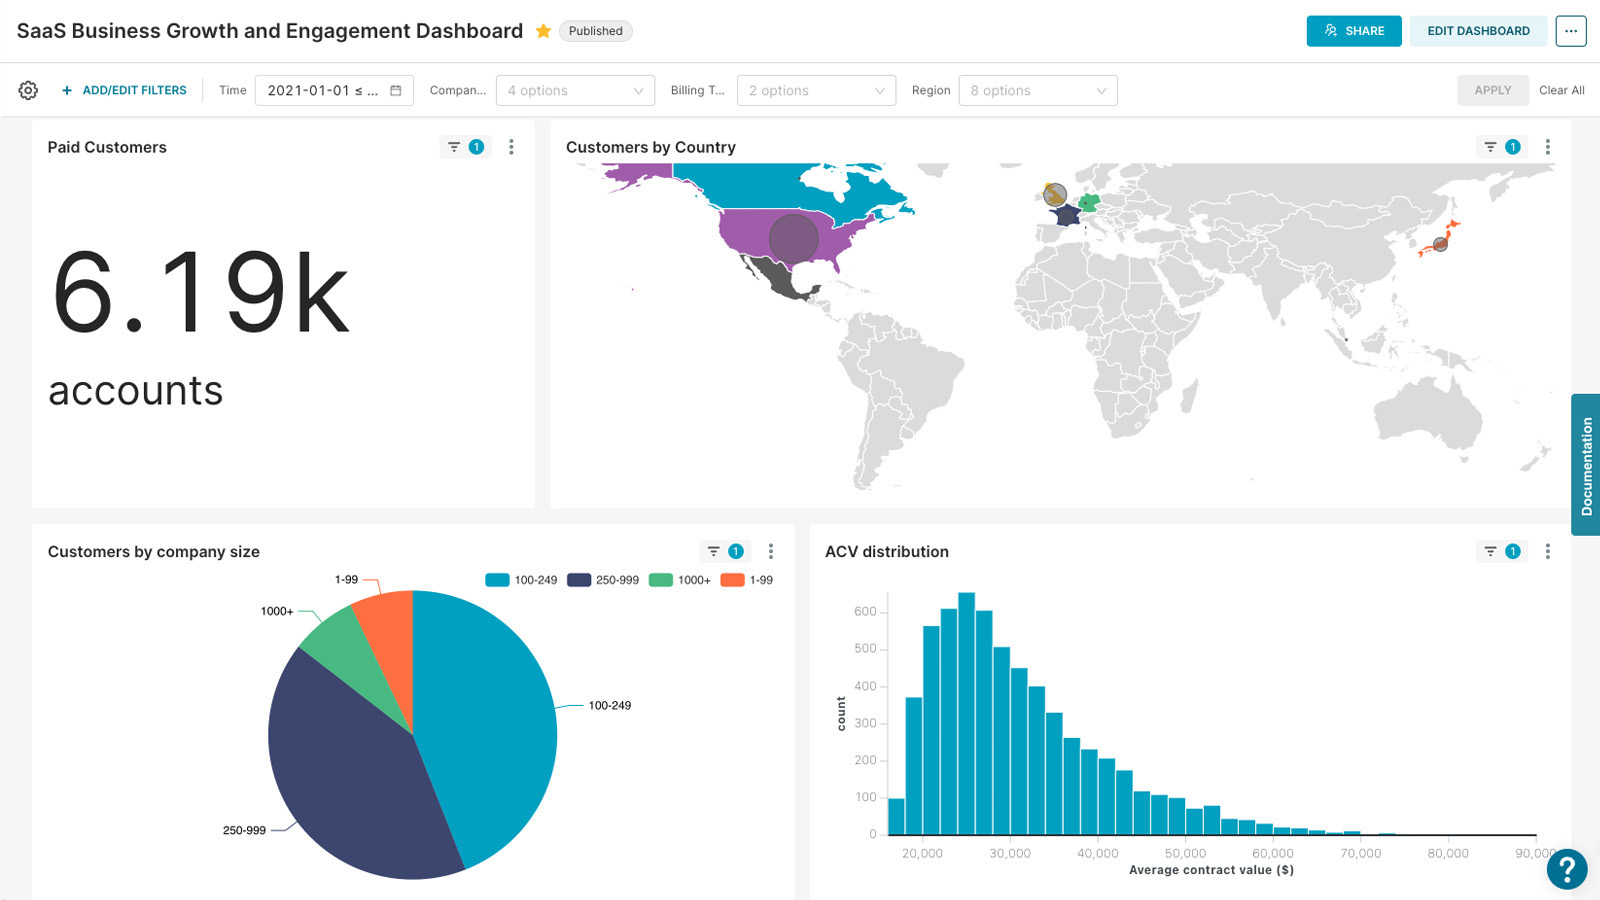
\includegraphics[width=0.9\textheight, angle=90]{figures/superset-dashboard.jpg}
    \caption{An example Apache Superset dashboard~\cite{ASF2024a}.}
    \label{fig:superset-dashboard}
\end{figure}

\begin{figure}[H]
    \centering
    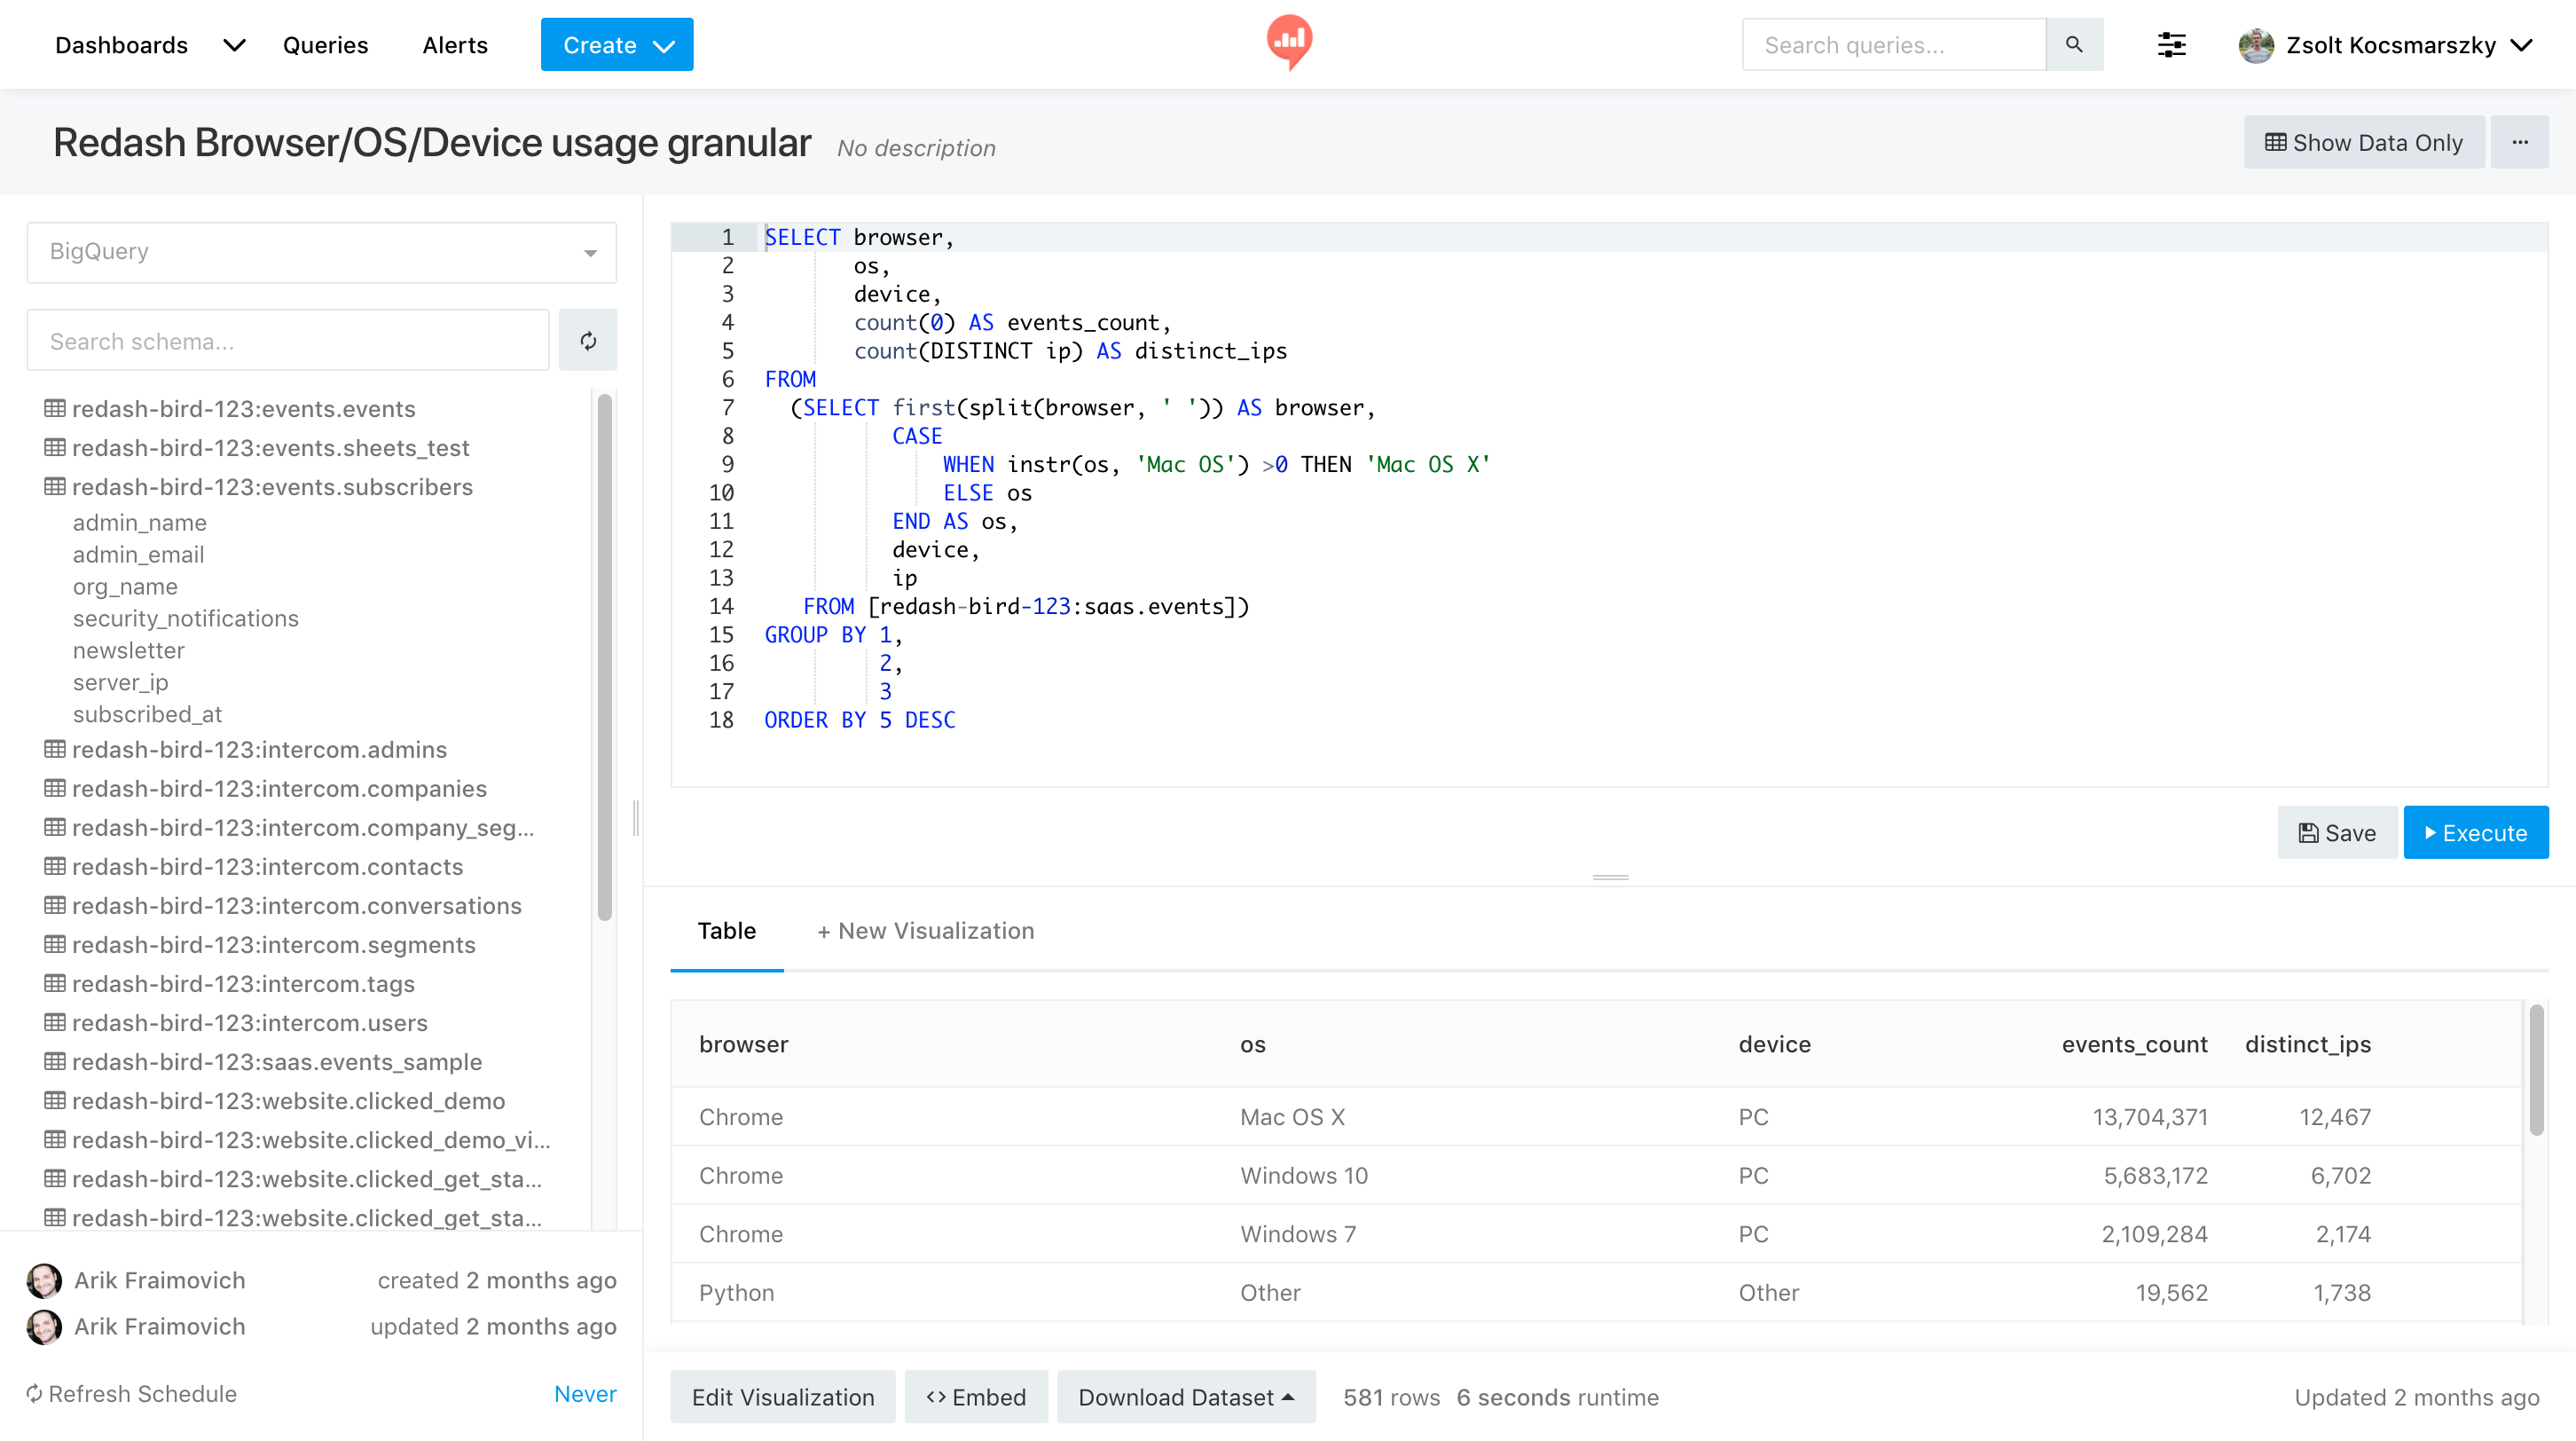
\includegraphics[width=0.9\textheight, angle=90]{figures/redash-query-editor.png}
    \caption{Redash's query editor~\cite{RedashCommunity2024}.}
    \label{fig:redash-query-editor}
\end{figure}

\begin{figure}[H]
    \centering
    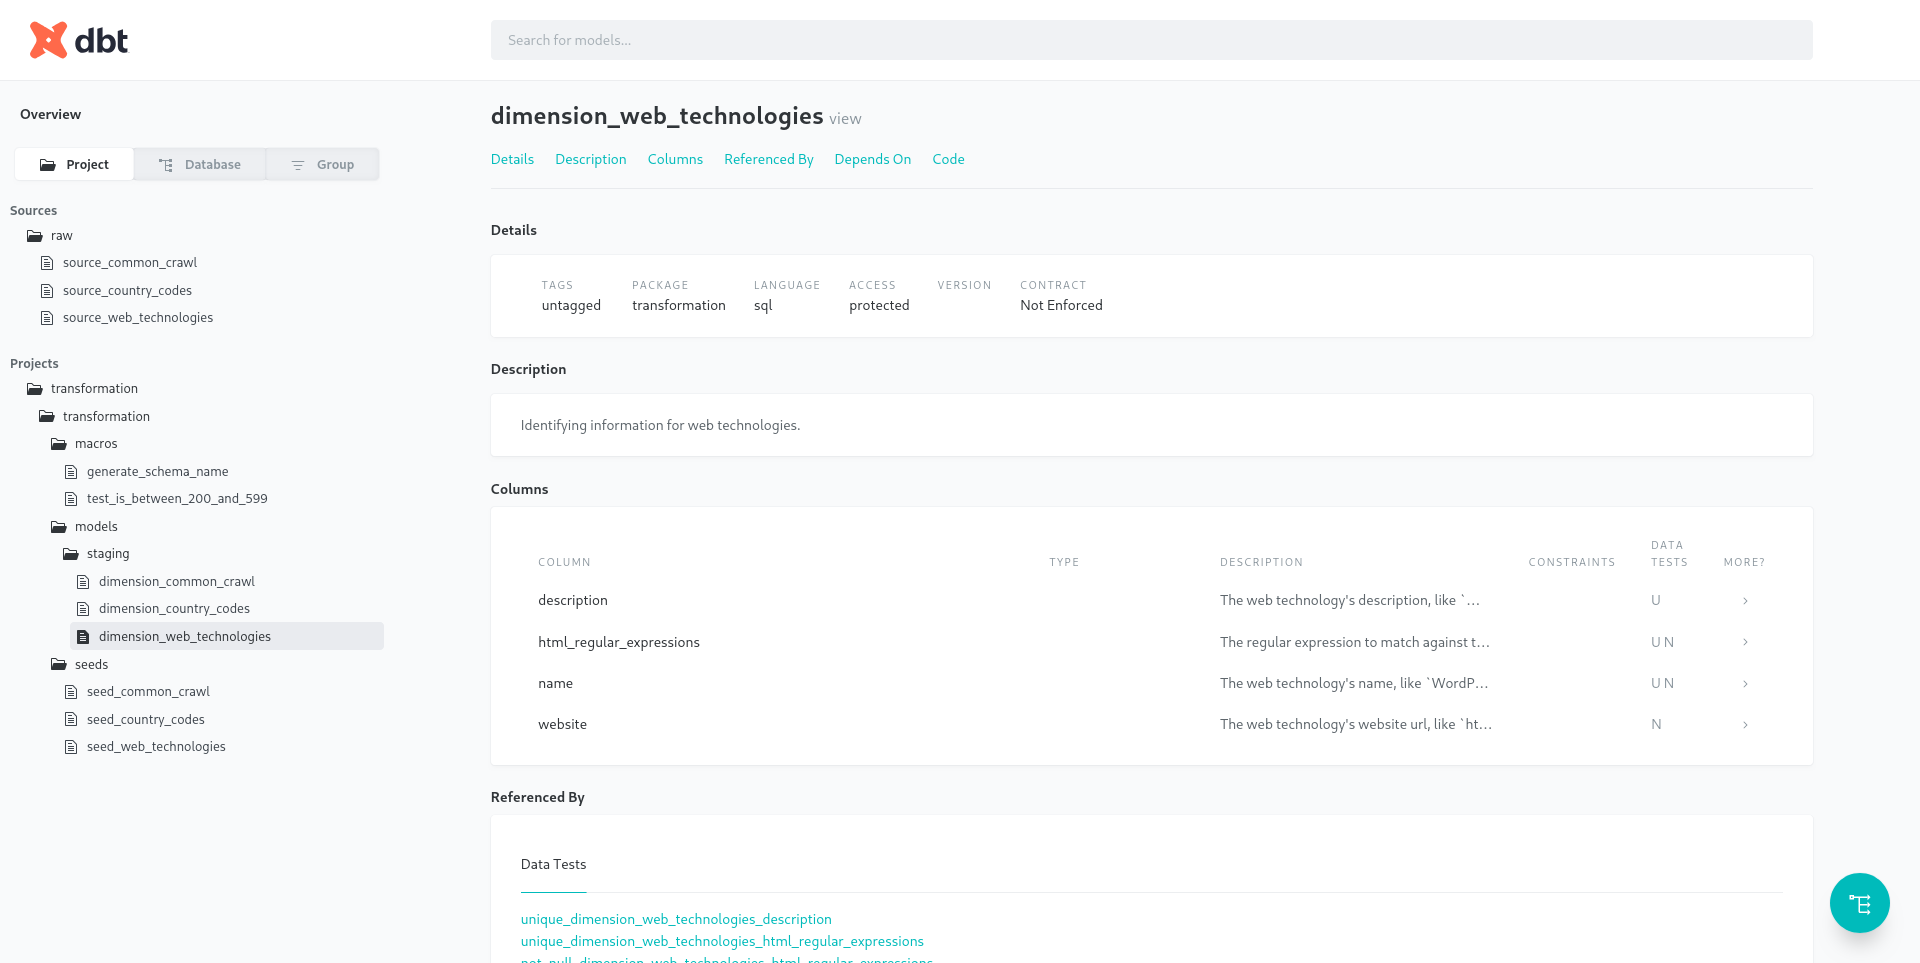
\includegraphics[width=0.9\textheight, angle=90]{figures/dbt-docs.png}
    \caption{Documentation of the dbt project.}
    \label{fig:appendix-guis-dbt-docs}
\end{figure}

\section{Local Kubernetes}
\label{sec:appendix-kubernetes}

Several Kubernetes distributions and virtualization environments support running Kubernetes locally.
\href{https://k3s.io/}{\textit{k3s}}, a certified Kubernetes distribution, is tailored for resource-constrained environments, which suits development contexts as opposed to multi-server production environments.
k3s can also run in Docker via a wrapper named \href{https://k3d.io/}{\textit{k3d}}.
The following command sets up a cluster with four namespaces in Kubernetes and a \href{https://traefik.io/traefik/}{\textit{Traefik}} ingress for external access to services:

\mint{sh}|k3d cluster create lakehouse|

Using the Kubernetes \ac{cli} \texttt{kubectl} and \href{https://helm.sh/}{\textit{Helm}} as the Kubernetes package manager, the installation of Longhorn (shown in \cref{lst:longhorn-setup}) fails.

\begin{listing}[H]
\begin{minted}{sh}
helm repo add longhorn https://charts.longhorn.io
helm repo update
helm install longhorn longhorn/longhorn --namespace longhorn-system --create-namespace
\end{minted}
\caption{Longhorn setup for Kubernetes using Helm.}
\label{lst:longhorn-setup}
\end{listing}

The issue arises because Longhorn relies on \ac{iscsi}, a protocol for connections and data transfers between computers and peripheral devices over \ac{tcp}, ``which cannot be installed in the standard k3s image, as it would have to use an OS base image''~\cite{Rizzi2021}.
According to a comment on the relevant feature request in k3d's \href{https://github.com/}{\textit{GitHub}} repository, creating a custom container image with a non-\texttt{scratch} OS base could resolve the issue.
However, this would be overly complex for our current needs.

Another local Kubernetes implementation is \href{https://minikube.sigs.k8s.io}{\textit{minikube}}, which can run on various drivers, including Docker and \acp{vm}.
To install the necessary \ac{iscsi} dependencies on an \ac{os}, we use the \ac{vm} driver as shown in \cref{lst:minikube-setup}.

\begin{listing}[H]
\begin{minted}{sh}
minikube start --driver=kvm2
minikube node add --worker
minikube ssh "sudo apt-get update;sudo apt-get install -y open-iscsi"
\end{minted}
\caption{Minikube setup using the VM driver.}
\label{lst:minikube-setup}
\end{listing}

Even though it is possible to install an \ac{iscsi} implementation, the service does not start, as \ac{iscsi} is also unsupported in minikube~\cite{Deutsch2017}.

The third and last option tested for a local Kubernetes setup was to use Rancher to create a Kubernetes cluster on Linux \acp{vm}.
Installing \texttt{open-iscsi} as above and deploying Longhorn through the Rancher \ac{gui} was initially successful.
However, issues arise when the cluster nodes reinitialize their availability, such as after waking from system hibernation, as Rancher becomes stuck waiting for the nodes to reconnect due to an ongoing bug~\cite{Henkens2023}.
This bug, opened in 2023, has since been closed due to inactivity.


\section{Supplementary Listings}
\label{sec:appendix-listings}

\begin{listing}[H]
\begin{minted}{bash}
#!/bin/bash
#
# Licensed to the Apache Software Foundation (ASF) under one
# or more contributor license agreements.  See the NOTICE file
# distributed with this work for additional information
# regarding copyright ownership.  The ASF licenses this file
# to you under the Apache License, Version 2.0 (the
# "License"); you may not use this file except in compliance
# with the License.  You may obtain a copy of the License at
#
#   http://www.apache.org/licenses/LICENSE-2.0
#
# Unless required by applicable law or agreed to in writing,
# software distributed under the License is distributed on an
# "AS IS" BASIS, WITHOUT WARRANTIES OR CONDITIONS OF ANY
# KIND, either express or implied.  See the License for the
# specific language governing permissions and limitations
# under the License.
set -e

start-master.sh -p 7077
# start-history-server.sh
start-thriftserver.sh  --driver-java-options "-Dderby.system.home=/tmp/derby"

# required for dbt
spark-sql <<EOF
CREATE DATABASE IF NOT EXISTS default;
EOF

# optional, to keep logs quiet
spark-sql <<EOF
CREATE DATABASE IF NOT EXISTS raw;
CREATE DATABASE IF NOT EXISTS staging;
CREATE DATABASE IF NOT EXISTS marts;
EOF

# Entrypoint, for example notebook, pyspark or spark-sql
if [[ $# -gt 0 ]] ; then
    eval "$1"
fi
\end{minted}
\caption{Entrypoint for the Spark master.}
\label{lst:spark-master-entrypoint}
\end{listing}

\begin{listing}[H]
\begin{minted}{bash}
#!/bin/bash
#
# Licensed to the Apache Software Foundation (ASF) under one
# or more contributor license agreements.  See the NOTICE file
# distributed with this work for additional information
# regarding copyright ownership.  The ASF licenses this file
# to you under the Apache License, Version 2.0 (the
# "License"); you may not use this file except in compliance
# with the License.  You may obtain a copy of the License at
#
#   http://www.apache.org/licenses/LICENSE-2.0
#
# Unless required by applicable law or agreed to in writing,
# software distributed under the License is distributed on an
# "AS IS" BASIS, WITHOUT WARRANTIES OR CONDITIONS OF ANY
# KIND, either express or implied.  See the License for the
# specific language governing permissions and limitations
# under the License.
set -e

pip install iso3166

start-worker.sh spark://spark-iceberg:7077 --port 8787
# start-history-server.sh

# Entrypoint, for example notebook, pyspark or spark-sql
if [[ $# -gt 0 ]] ; then
    eval "$1"
fi
\end{minted}
\caption{Entrypoint for a Spark worker.}
\label{lst:spark-worker-entrypoint}
\end{listing}

\begin{listing}[H]
\begin{minted}{bash}
#
# Licensed to the Apache Software Foundation (ASF) under one or more
# contributor license agreements.  See the NOTICE file distributed with
# this work for additional information regarding copyright ownership.
# The ASF licenses this file to You under the Apache License, Version 2.0
# (the "License"); you may not use this file except in compliance with
# the License.  You may obtain a copy of the License at
#
#    http://www.apache.org/licenses/LICENSE-2.0
#
# Unless required by applicable law or agreed to in writing, software
# distributed under the License is distributed on an "AS IS" BASIS,
# WITHOUT WARRANTIES OR CONDITIONS OF ANY KIND, either express or implied.
# See the License for the specific language governing permissions and
# limitations under the License.
#

# Default system properties included when running spark-submit.
# This is useful for setting default environmental settings.

spark.sql.extensions                        org.apache.iceberg.spark.extensions.IcebergSparkSessionExtensions
spark.sql.catalog.demo                      org.apache.iceberg.spark.SparkCatalog
spark.sql.catalog.demo.type                 rest
spark.sql.catalog.demo.uri                  http://rest:8181
spark.sql.catalog.demo.io-impl              org.apache.iceberg.aws.s3.S3FileIO
spark.sql.catalog.demo.s3.endpoint          http://minio:9000
spark.sql.catalog.demo.s3.path-style-access true
spark.sql.defaultCatalog                    demo
spark.eventLog.enabled                      true
spark.eventLog.dir                          /home/iceberg/spark-events
spark.history.fs.logDirectory               /home/iceberg/spark-events
spark.sql.catalogImplementation             in-memory
\end{minted}
\caption{Spark's default configuration.}
\label{lst:spark-defaults}
\end{listing}

\begin{listing}[H]
\begin{minted}{yaml}
services:
  minio:
    environment:
      MINIO_DOMAIN: minio
    networks:
      default:
        aliases:
        - lakehouse.minio
\end{minted}
\caption{Docker Compose configuration for MinIO's Virtual Host access style.}
\label{lst:compose-mino-virtual-host}
\end{listing}

\begin{listing}[H]
\begin{minted}{python}
@measure_performance
def fetch_warc_datasets():
  url = "https://index.commoncrawl.org/collinfo.json"
  response = requests.get(url)
  response.raise_for_status()
  datasets = response.json()

  if not datasets:
    raise ValueError("No datasets found.")

  return datasets


@measure_performance
def fetch_warc_paths(dataset_id: str, dataset_subset: str = 'warc'):
  url = urljoin(
    "https://data.commoncrawl.org/",
    f"crawl-data/{dataset_id}/{dataset_subset}.paths.gz",
  )
  response = requests.get(url)
  response.raise_for_status()

  warc_paths = (
    gzip.decompress(response.content)
    .decode("utf-8")
    .splitlines()
  )

  if not warc_paths:
    raise ValueError("No WARC paths found.")

  return warc_paths


@retry(
    stop=stop_after_attempt(5),
    wait=wait_exponential(min=1, max=10),
)
@measure_performance
def fetch_warc_stream(warc_file: str):
  url = urljoin("https://data.commoncrawl.org/", warc_file)
  response = requests.get(url, stream=True)
  response.raise_for_status()

  return response
\end{minted}
\caption{Network utility functions for Common Crawl ingestion.}
\label{lst:dagster-source-common-crawl-fetch}
\end{listing}


\begin{listing}[H]
\begin{minted}{python}
def measure_performance(func):
  def wrapper(*args, **kwargs):
    start_time = time.perf_counter()
    result = func(*args, **kwargs)
    end_time = time.perf_counter()
    elapsed_time = end_time - start_time
    logger.info(f"Time to execute {func.__name__}: {elapsed_time:.4f} seconds")
    return result

  return wrapper
\end{minted}
\caption{Decorator for performance measurement.}
\label{lst:dagster-utility-performance-measurement}
\end{listing}


\begin{listing}[H]
\begin{minted}{python}
def batch_records(
  data: Generator,
  max_batch_size=134217728, # bytes = 128 MiB
):
  counter = 0
  batch = []
  batch_size = 0

  for record in data:
    record_size = asizeof.asizeof(record)

    if batch_size + record_size > max_batch_size:
      if batch:
        yield batch
        batch = []
        batch_size = 0

    batch.append(record)
    batch_size += record_size
    counter += 1

  if batch:
    yield batch
\end{minted}
\caption{Batching algorithm for records up to a specified batch size.}
\label{lst:dagster-utility-performance-batching}
\end{listing}


\begin{listing}[H]
\begin{minted}{python}
BUFFER_SIZE = 5


async def batch_process(
  data_stream: Generator,
  func: Callable[[List[dict], bool], None]
):
  is_written = False
  buffer = asyncio.Queue(maxsize=BUFFER_SIZE)

  async def producer():
    for batch in data_stream:
      await buffer.put(batch)

    await buffer.put(None)

  async def fetch_next_item():
    try:
      batch = next(data_stream)
      await buffer.put(batch)
    except StopIteration:
      await buffer.put(None)

  async def consumer():
    nonlocal is_written
    while True:
      batch = await buffer.get()

      if batch is None:
        buffer.task_done()
        await buffer.put(None)
        break

      func(batch, is_written)

      if not is_written:
        is_written = True

      buffer.task_done()

      if buffer.qsize() < BUFFER_SIZE:
        await fetch_next_item()

  initial_fill = [fetch_next_item() for _ in range(BUFFER_SIZE)]
  await asyncio.gather(*initial_fill)
  await consumer()
\end{minted}
\caption{Queuing algorithm for processing batches with a specified buffer size.}
\label{lst:dagster-utility-performance-queuing}
\end{listing}

\begin{listing}[H]
\begin{minted}{python}
MEMORY = "50g" if IS_KUBERNETES else "4g"


class SparkSingleton:
  def __init__(self):
    self._spark = None

  @property
  def spark(self):
    if self._spark is None:
      self._spark = (
        SparkSession.builder.appName("Big Data Pipeline")
        .master("spark://spark-iceberg:7077")
        .config("spark.driver.host", "dagster")
        .config("spark.driver.bindAddress", "0.0.0.0")
        .config("spark.driver.memory", MEMORY)
        .config("spark.driver.port", "7777")
        .config("spark.blockManager.port", "7878")
        .config("spark.executor.memory", MEMORY)
        .config("spark.rpc.message.maxSize", "1024")
        .config(
          "spark.jars.packages",
          "org.apache.iceberg:iceberg-spark-runtime-3.5_2.12:1.6.1,"
          "org.apache.iceberg:iceberg-aws-bundle:1.6.1",
        )
        .config(
          "spark.sql.extensions",
          "org.apache.iceberg.spark.extensions.IcebergSparkSessionExtensions",
        )
        .config("spark.sql.catalog.demo", "org.apache.iceberg.spark.SparkCatalog")
        .config("spark.sql.catalog.demo.type", "rest")
        .config("spark.sql.catalog.demo.uri", "http://rest:8181")
        .config("spark.sql.catalog.demo.io-impl", "org.apache.iceberg.aws.s3.S3FileIO")
        .config("spark.sql.catalog.demo.s3.endpoint", "http://minio:9000")
        .config("spark.sql.catalog.demo.s3.path-style-access", "true")
        .config("spark.sql.defaultCatalog", "demo")
        .config("spark.sql.catalogImplementation", "in-memory")
        .getOrCreate()
      )
    return self._spark


SparkManager = SparkSingleton()
\end{minted}
\caption{\texttt{SparkSession} defined as a singleton.}
\label{lst:dagster-utility-spark}
\end{listing}

\begin{listing}[H]
\begin{minted}{python}
TABLE = "raw.source_common_crawl"


def write_source(batch: list):
  if not SparkManager.spark.catalog.tableExists(TABLE):
    SparkManager.spark.sql(f"""
      CREATE TABLE {TABLE} (
        dataset_id string NOT NULL,
        response_charset string,
        response_headers_status_code integer NOT NULL,
        response_payload string NOT NULL,
        response_payload_size_bytes integer NOT NULL,
        response_payload_length integer NOT NULL,
        response_target_uri string NOT NULL
      )
      USING iceberg
      PARTITIONED BY (dataset_id, response_charset)
    """)
    SparkManager.spark.sql(
      f"ALTER TABLE {TABLE} SET IDENTIFIER FIELDS dataset_id, response_target_uri"
    )

  dataframe = SparkManager.spark.createDataFrame(batch)
  existing_data = SparkManager.spark.table(TABLE)
  new_rows = dataframe.join(
    existing_data,
    on=(dataframe["dataset_id"] == existing_data["dataset_id"])
    & (dataframe["response_target_uri"] == existing_data["response_target_uri"]),
    how="left_anti",
  )
  new_rows.writeTo(TABLE).append()
\end{minted}
\caption{Appending deduplicated entries to a partitioned Iceberg table.}
\label{lst:dagster-source-common-crawl-write-deduplicated}
\end{listing}

\begin{listing}[H]
\begin{minted}{jinja}

Data from one of the largest public web crawling datasets.



The HTTP status code of the response, such as `200`.

\end{minted}
\caption{Definition of documentation in dbt.}
\label{lst:appendix-listings-dbt-doc}
\end{listing}

\begin{listing}[H]
\begin{minted}{sh}
poetry run dbt docs generate
poetry run dbt docs serve
\end{minted}
\caption{Commands to generate and serve dbt project documentation.}
\label{lst:implementation-pipeline-transformation-dbt-docs}
\end{listing}

\begin{listing}[H]
\begin{minted}{python}
COUNTRY_CODES_URL = "https://en.wikipedia.org/wiki/List_of_ISO_3166_country_codes"
MODULE_NAME = "country_codes"


def fetch_tables() -> list[pandas.DataFrame]:
  # without `keep_default_na`, the country code for Namibia (`NA`) would be parsed as `NoneType`
  tables = pandas.read_html(COUNTRY_CODES_URL, keep_default_na=False)
  return tables
\end{minted}
\caption{Basic table extraction using Pandas.}
\label{lst:appendix-listings-pandas-tables}
\end{listing}

\begin{listing}[H]
\begin{minted}{bash}
FROM python:3.11.9 AS base-image
ENV CI=true
ENV PYTHONUNBUFFERED=1
ENV DAGSTER_HOME=/home/rootless/dagster
WORKDIR /srv/app/
# ... install poetry, add user `rootless` ...
USER rootless:rootless
RUN mkdir /home/rootless/dagster \
  && touch /home/rootless/dagster/dagster.yaml \
  && poetry config virtualenvs.in-project true

FROM base-image AS development
COPY ./docker/dagster/entrypoint.sh /usr/local/bin/docker-entrypoint.sh
ENTRYPOINT ["docker-entrypoint.sh"]
CMD ["poetry", "run", "dagster", "dev", "--host", "0.0.0.0"]
VOLUME /srv/app
VOLUME /srv/charts
VOLUME /srv/transformation
EXPOSE 3000

FROM base-image AS prepare
COPY --chown=rootless ./orchestration/pyproject.toml ./orchestration/poetry.lock ./orchestration/
WORKDIR /srv/app/orchestration
RUN poetry install

FROM prepare AS build
WORKDIR /srv/app
COPY --chown=rootless ./orchestration ./orchestration
COPY --chown=rootless ./transformation ./transformation
WORKDIR /srv/app/orchestration
RUN poetry run dagster-dbt project prepare-and-package --file orchestration/project.py

FROM build AS production
ENV DAGSTER_DEPLOYMENT=production
USER root:root
# ... install updates ...
USER rootless:rootless
CMD ["poetry", "run", "dagster-webserver", "--host", "0.0.0.0"]
VOLUME /srv/charts
EXPOSE 3000
\end{minted}
\caption{Multistage Dockerfile for the Big Data pipeline.}
\label{lst:appendix-listings-dockerfile}
\end{listing}

\begin{listing}[H]
\begin{minted}{text}
INFO:root:Time to execute fetch_warc_datasets: 0.3882 seconds
INFO:root:Time to execute fetch_warc_paths: 0.1251 seconds
INFO:root:Processing path "crawl-data/CC-MAIN-2024-42/segments/1727944253146.59/warc/ CC-MAIN-20241003094020-20241003124020-00000.warc.gz"
INFO:root:Time to execute fetch_warc_stream: 0.6644 seconds
INFO:root:Time to execute get_warc_record_stream: 0.0000 seconds
org.apache.iceberg#iceberg-spark-runtime-3.5_2.12 added as a dependency
org.apache.iceberg#iceberg-aws-bundle added as a dependency
:: resolving dependencies :: org.apache.spark#spark-submit-parent-6ac38175-0b5c-4e68-a308-36539b91fc31; 1.0
    confs: [default]
    found org.apache.iceberg#iceberg-spark-runtime-3.5_2.12;1.6.1 in central
    found org.apache.iceberg#iceberg-aws-bundle;1.6.1 in central
:: resolution report :: resolve 174ms :: artifacts dl 6ms
    :: modules in use:
    org.apache.iceberg#iceberg-aws-bundle;1.6.1 from central in [default]
    org.apache.iceberg#iceberg-spark-runtime-3.5_2.12;1.6.1 from central in [default]
    ---------------------------------------------------------------------
    |                  |            modules            ||   artifacts   |
    |       conf       | number| search|dwnlded|evicted|| number|dwnlded|
    ---------------------------------------------------------------------
    |      default     |   2   |   0   |   0   |   0   ||   2   |   0   |
    ---------------------------------------------------------------------
:: retrieving :: org.apache.spark#spark-submit-parent-6ac38175-0b5c-4e68-a308-36539b91fc31
    confs: [default]
    0 artifacts copied, 2 already retrieved (0kB/6ms)
WARN TaskSetManager: Stage 0 contains a task of very large size (3827 KiB).  The maximum recommended task size is 1000 KiB.
INFO:root:Time to execute write_source: 68.0258 seconds
WARN TaskSetManager: Stage 6 contains a task of very large size (3182 KiB).  The maximum recommended task size is 1000 KiB.
INFO:root:Time to execute write_source: 42.6831 seconds
WARN TaskSetManager: Stage 12 contains a task of very large size (2918 KiB). The maximum recommended task size is 1000 KiB.
INFO:root:Time to execute write_source: 38.4028 seconds
WARN TaskSetManager: Stage 18 contains a task of very large size (3283 KiB). The maximum recommended task size is 1000 KiB.
INFO:root:Time to execute write_source: 37.8254 seconds
# ...
WARN TaskSetManager: Stage 48 contains a task of very large size (1679 KiB). The maximum recommended task size is 1000 KiB.
INFO:root:Time to execute write_source: 35.3250 seconds
\end{minted}
\caption{Simplified asset job logs for Common Crawl ingestion.}
\label{lst:appendix-listings-spark-logs}
\end{listing}


\clearpage
\section{Spark Driver}
\label{sec:appendix-spark}

\begin{figure}[H]
    \centering
    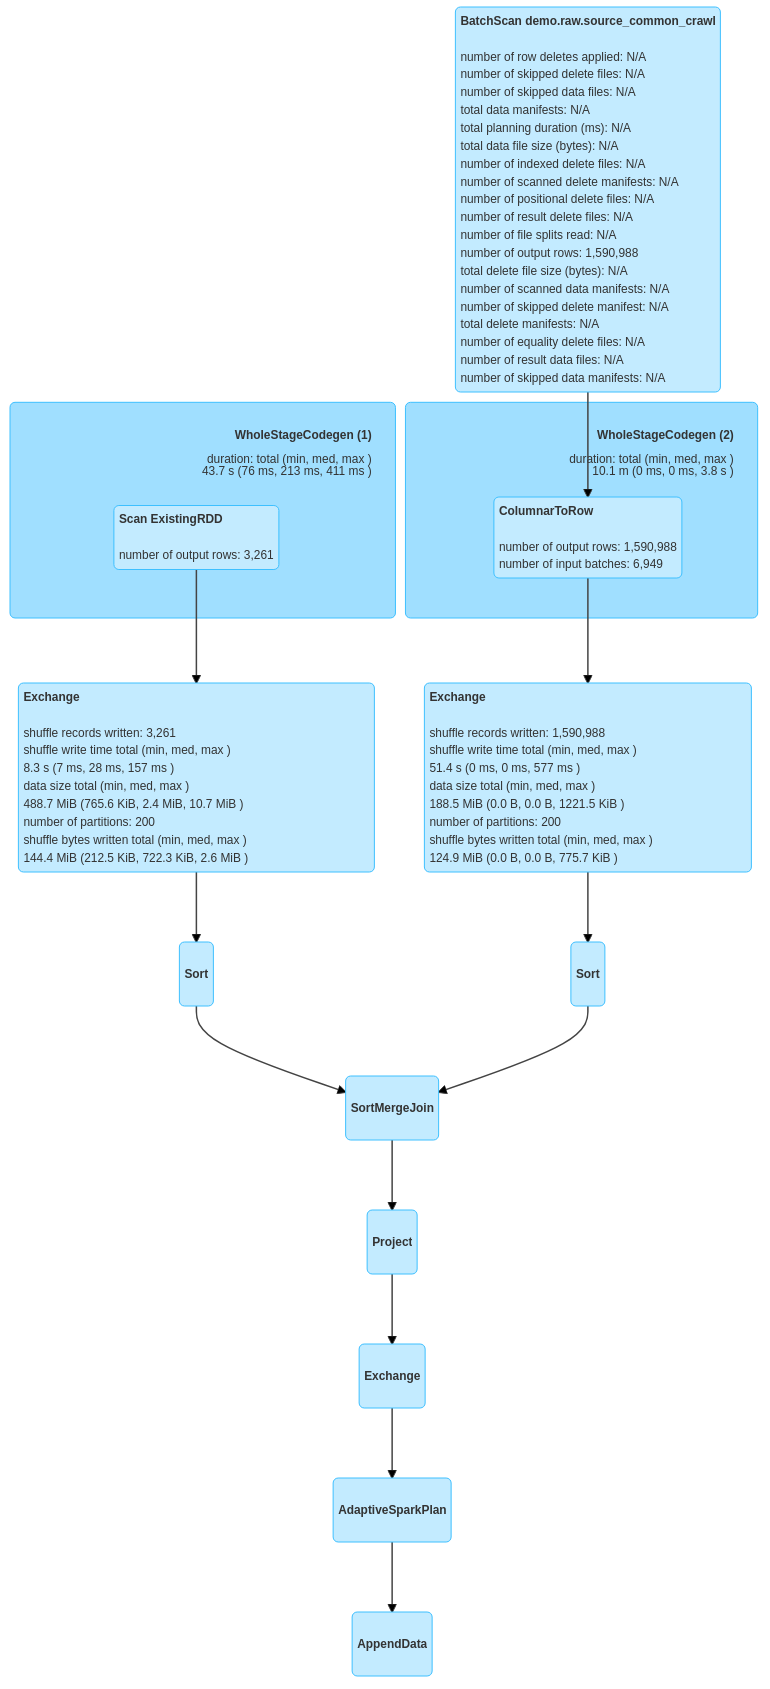
\includegraphics[height=0.9\textheight]{figures/driver-query.png}
    \caption{Spark driver's query diagram for appending data.}
    \label{fig:analysis-pipeline-performance-driver}
\end{figure}


\clearpage
\section{Overall Port List}
\label{sec:appendix-ports}

\begin{table}[H]
    \centering
    \begin{tabular}{|c|c|c|c|}
    \hline
    \textbf{Port} & \textbf{Application} & \textbf{Type} & \textbf{Component} \\
    \hline
    3000 & Dagster & GUI & ~ \\
    \hline
    3001 & Charts & GUI & ~ \\
    \hline
    4040 & Spark & GUI & Driver \\
    \hline
    7077 & Spark & API & Master \\
    \hline
    7777 & Spark & API & Driver \\
    \hline
    7878 & Spark & API & Block Manager \\
    \hline
    8080 & Jupyter Notebook & GUI & ~ \\
    \hline
    8181 & Iceberg & API & REST Catalog \\
    \hline
    8888 & Spark & GUI & Master \\
    \hline
    9000 & MinIO & API & ~ \\
    \hline
    9001 & MinIO & GUI & ~ \\
    \hline
    10000 & Thrift & API & ~ \\
    \hline
    \end{tabular}
    \caption{List of ports and their respective applications.}
    \label{tab:appendix-ports}
\end{table}


\clearpage
\section{Large Charts}
\label{sec:appendix-charts}

\begin{figure}[H]
    \centering
    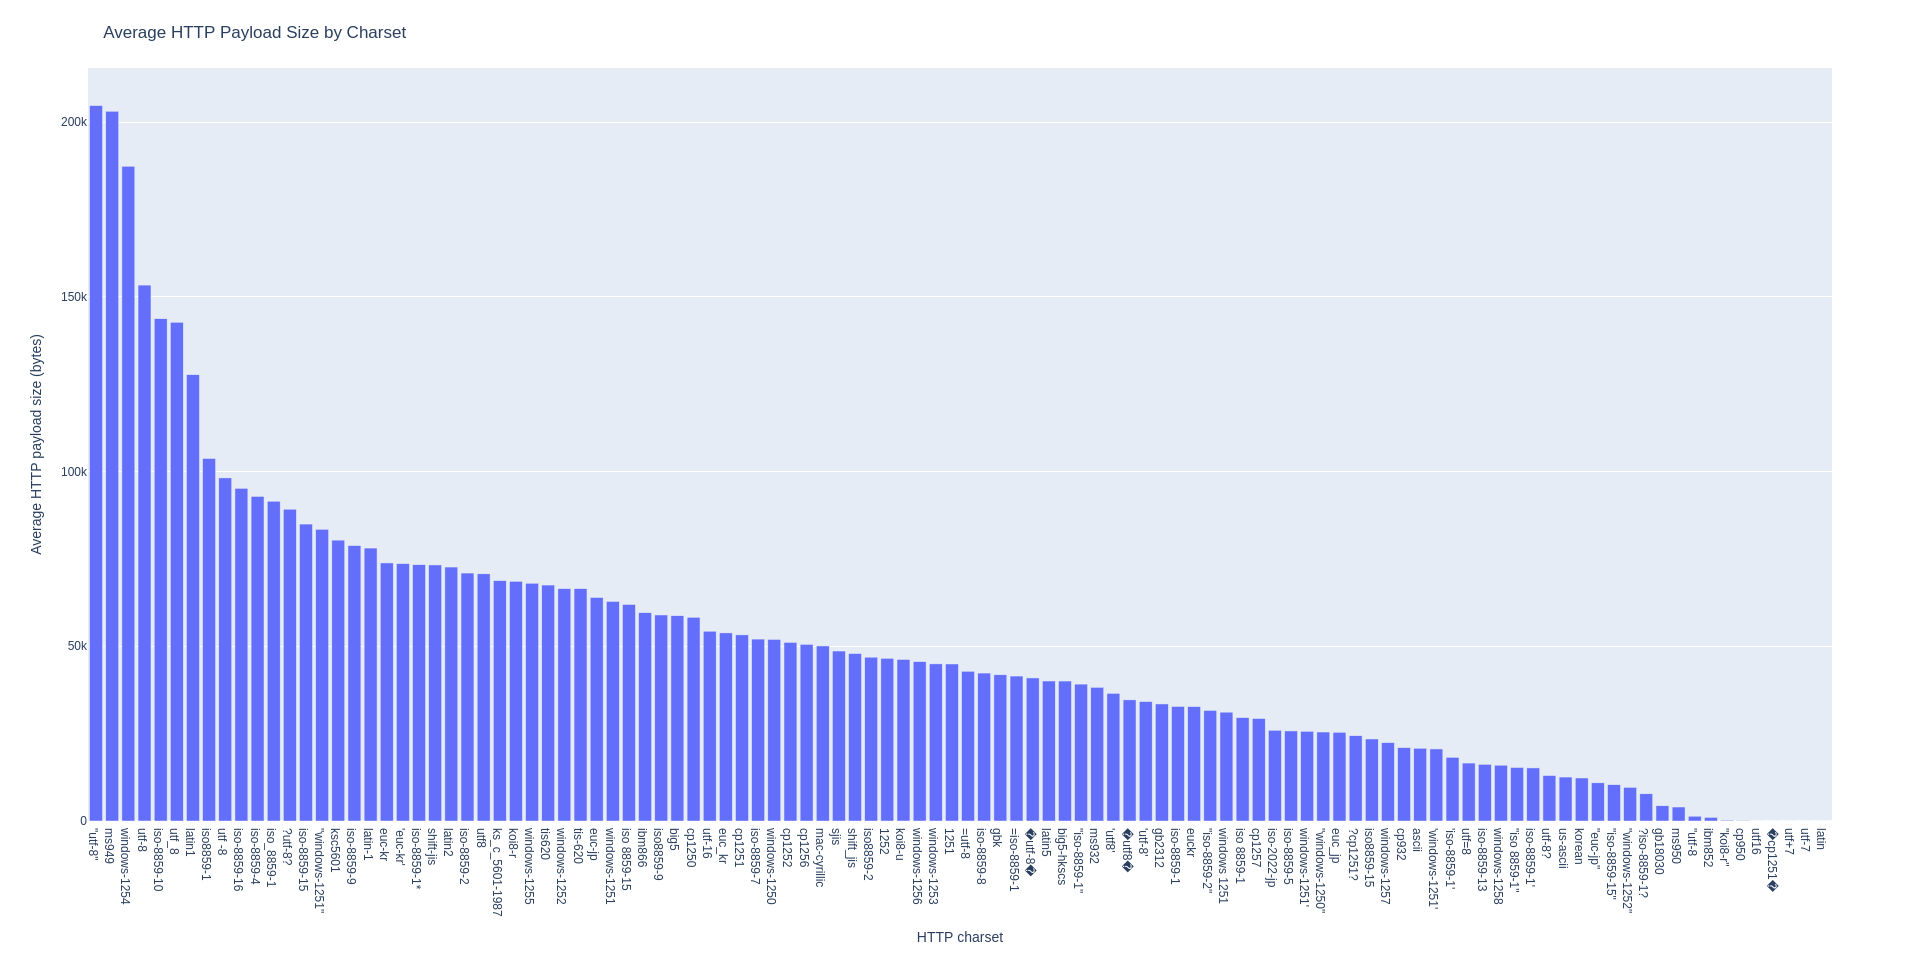
\includegraphics[width=0.9\textheight, angle=90]{figures/charts/large/appendix/chart_source_charset_bar_payload_size.png}
    \caption{Average payload size by charset.}
    \label{fig:analysis-dataset-chart_source_charset_bar_payload_size}
\end{figure}

\begin{figure}[H]
    \centering
    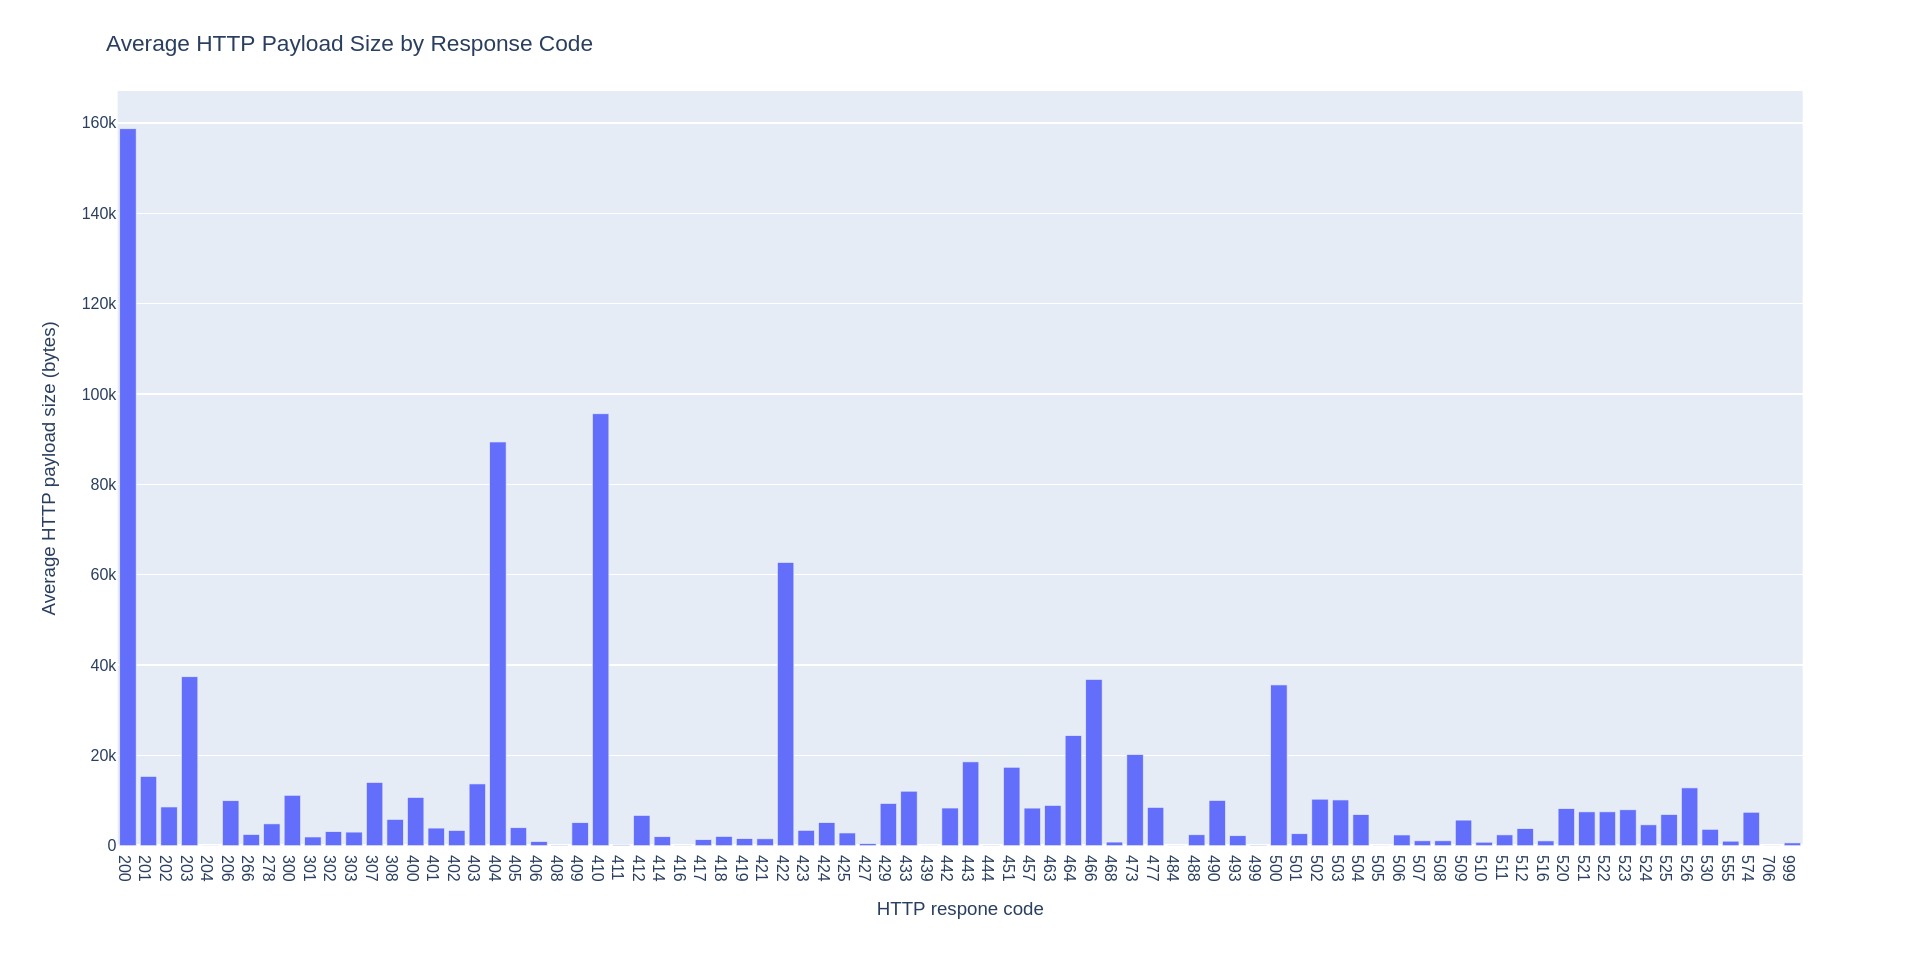
\includegraphics[width=\textheight, angle=90]{figures/charts/large/appendix/chart_source_response_code_bar_payload_size.png}
    \caption{Average payload size by response code.}
    \label{fig:analysis-dataset-chart_source_response_code_bar_payload_size}
\end{figure}

\begin{figure}[H]
    \centering
    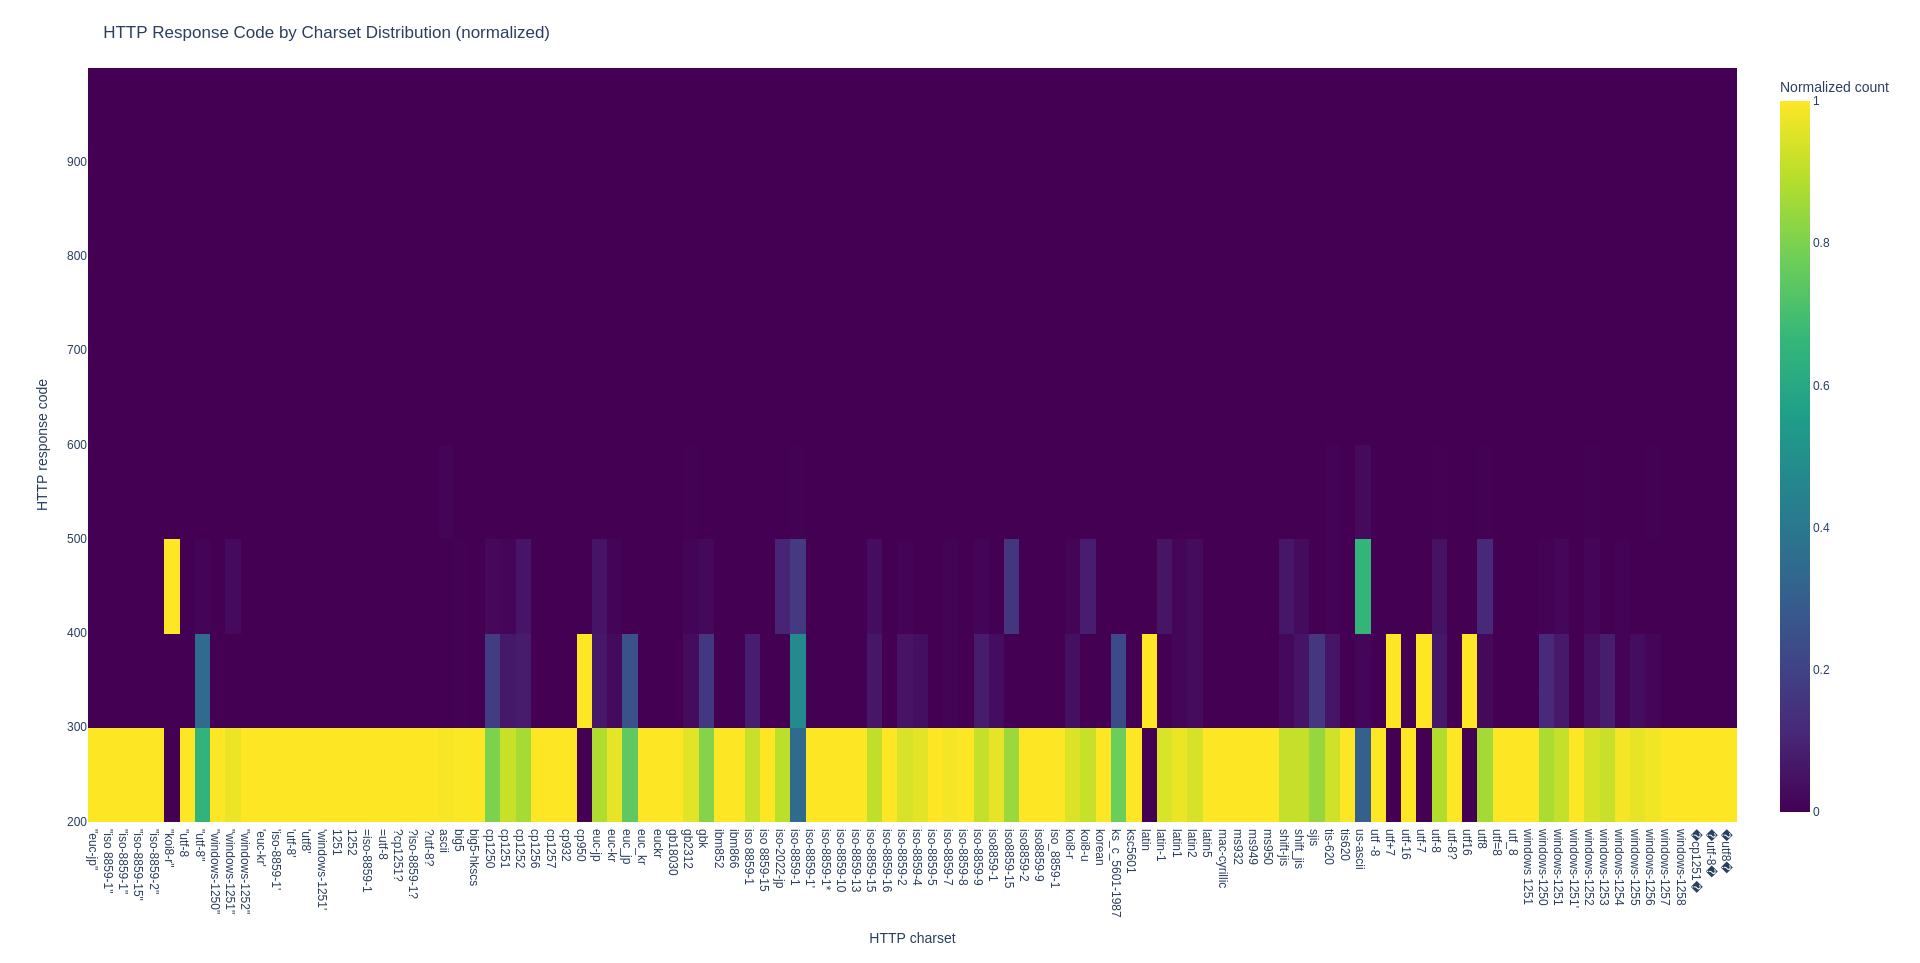
\includegraphics[width=\textheight, angle=90]{figures/charts/large/appendix/chart_source_charset_heatmap_response_code.png}
    \caption{Normalized response code distribution by charset.}
    \label{fig:analysis-dataset-chart_source_charset_heatmap_response_code}
\end{figure}

\begin{figure}[H]
    \centering
    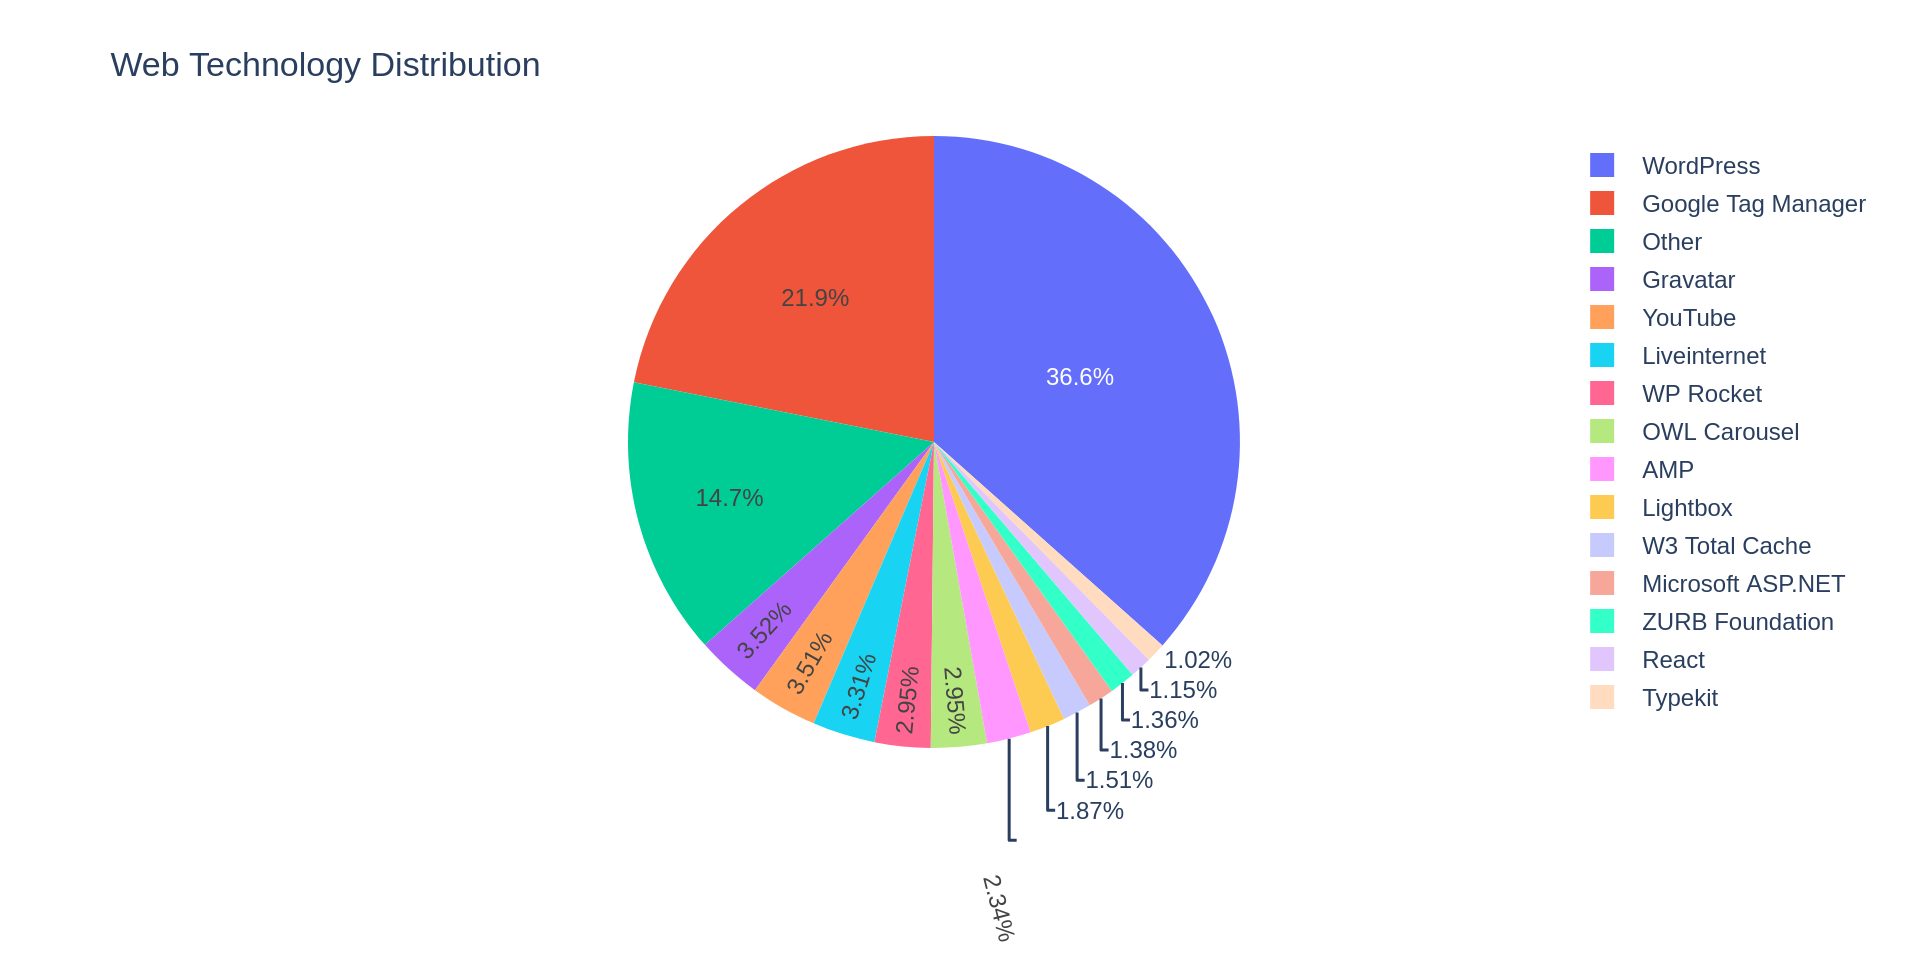
\includegraphics[width=\textheight, angle=90]{figures/charts/large/appendix/chart_fact_web_technology_pie.png}
    \caption{Distribution of web technologies.}
    \label{fig:analysis-dataset-chart_fact_web_technology_pie}
\end{figure}

\begin{figure}[H]
  \centering
  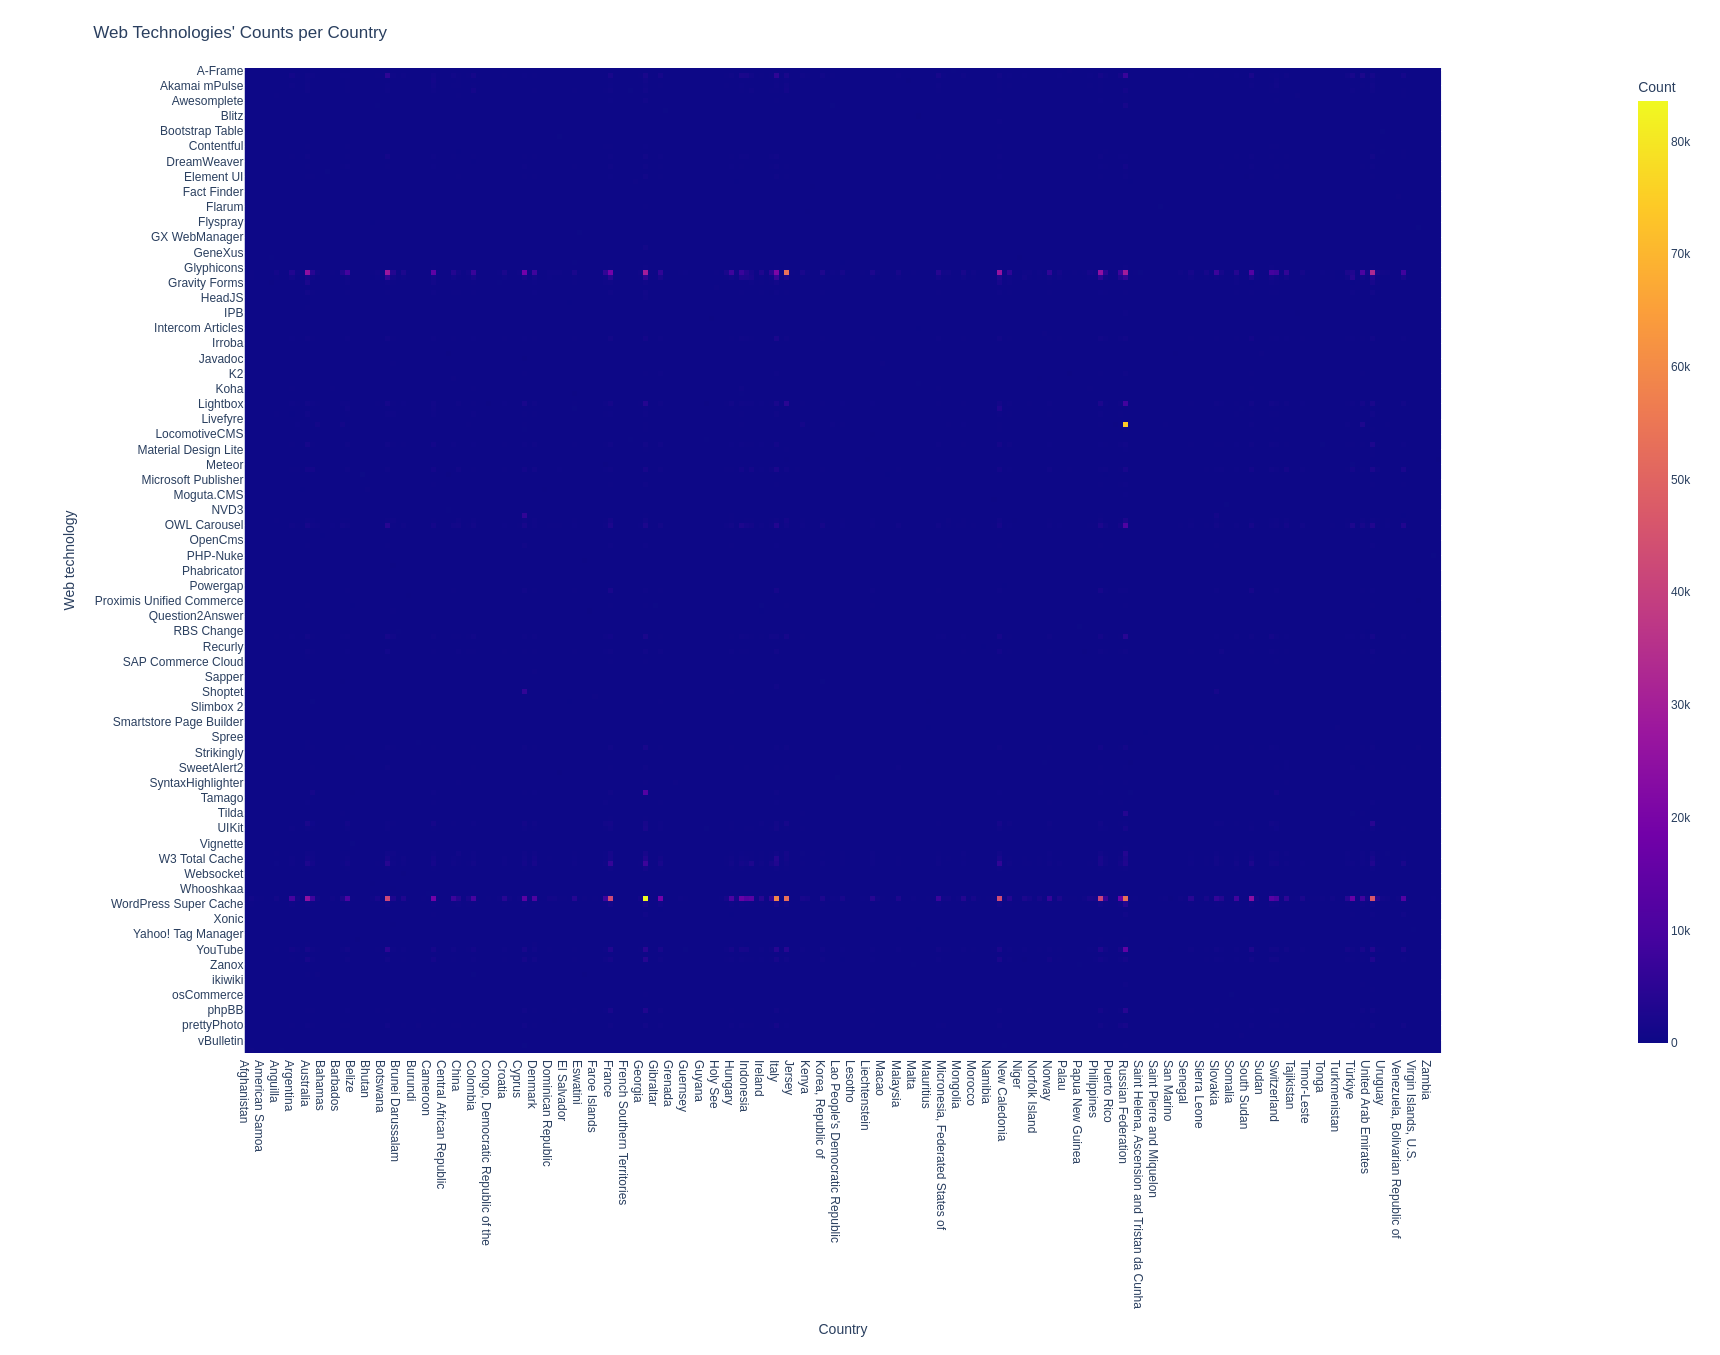
\includegraphics[height=\textwidth, angle=90]{figures/charts/large/appendix/chart_fact_web_technology_heatmap_country.png}
  \caption{Web technologies count per country.}
  \label{fig:analysis-dataset-chart_fact_web_technology_heatmap_country}
\end{figure}

\begin{figure}[H]
  \centering
  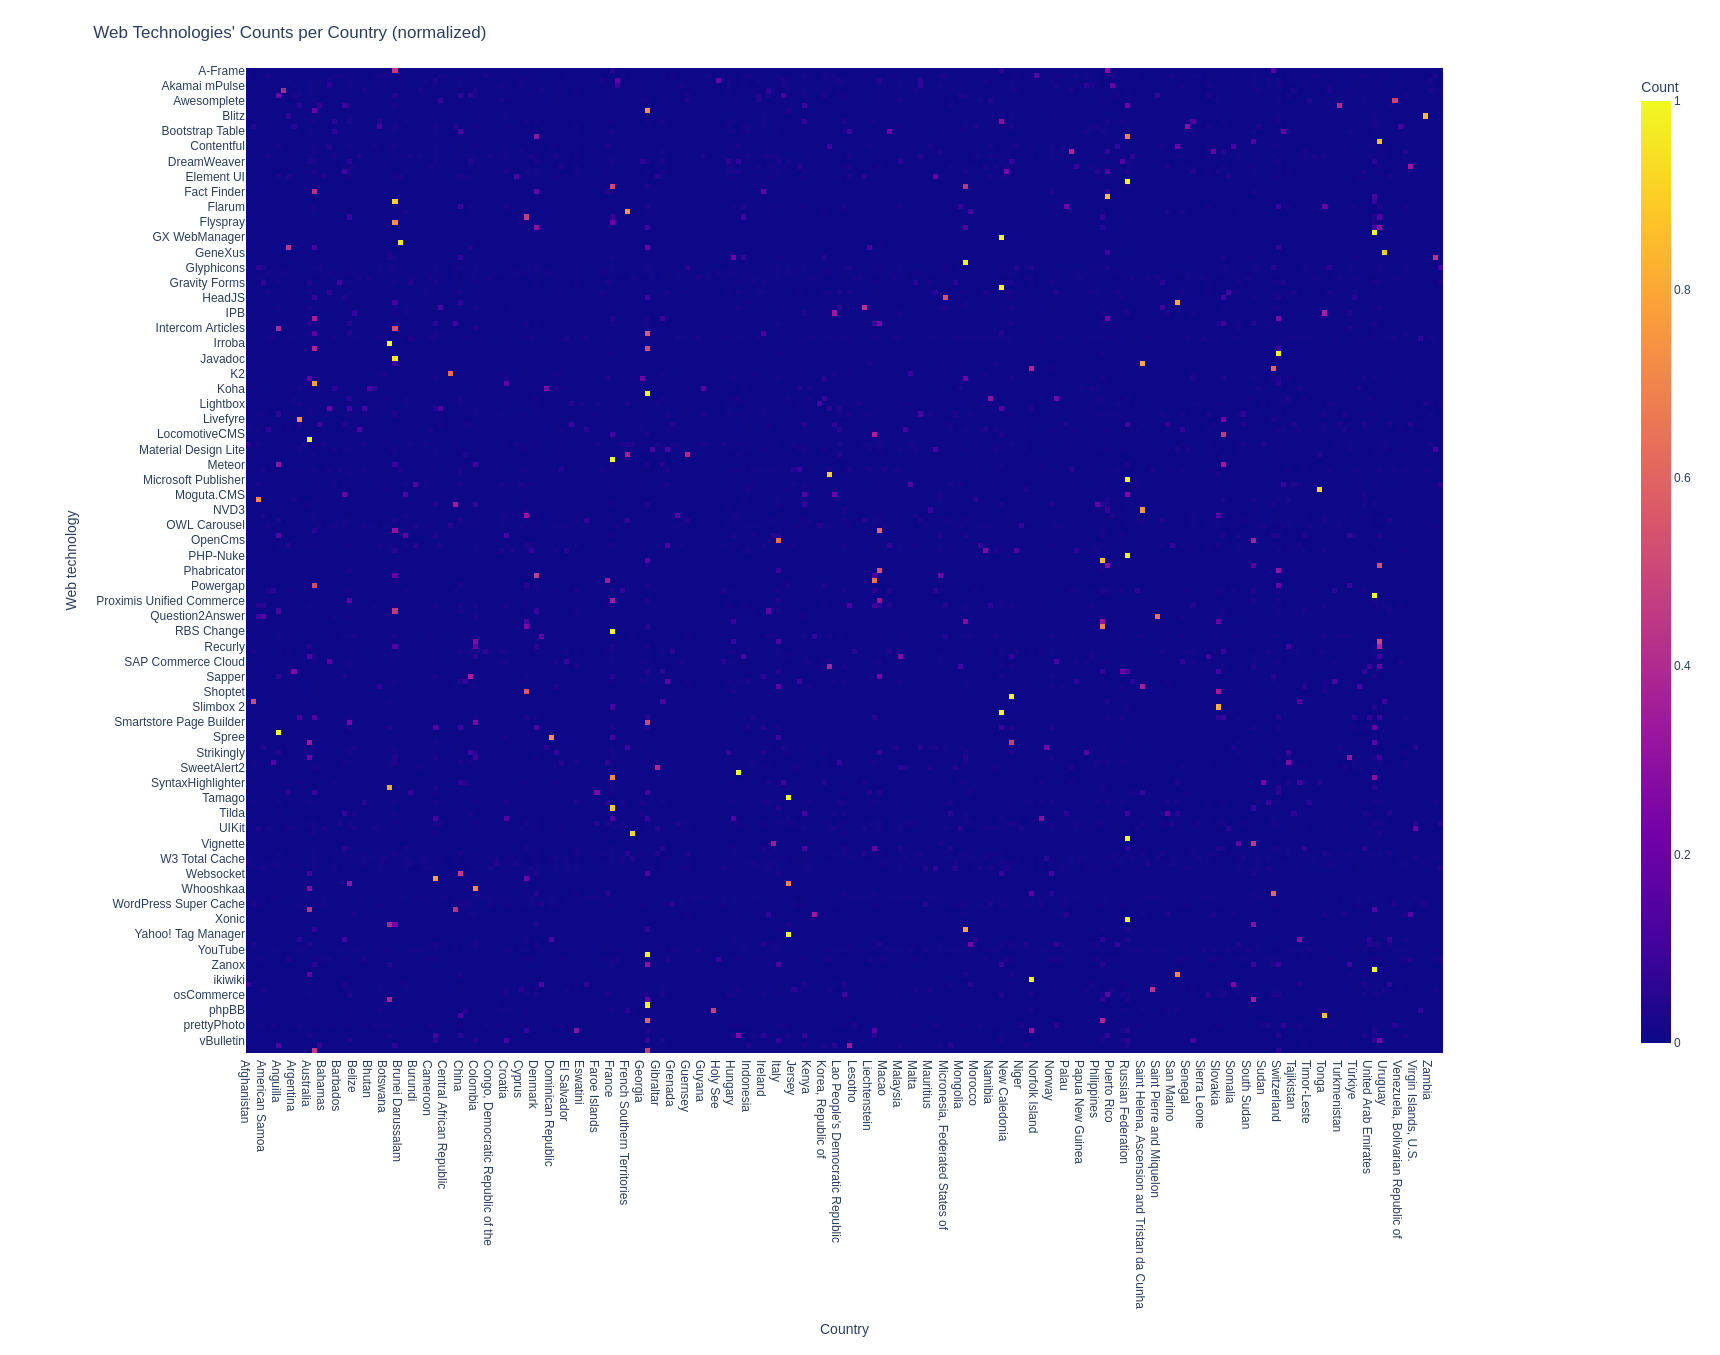
\includegraphics[height=\textwidth, angle=90]{figures/charts/large/appendix/chart_fact_web_technology_heatmap_country_normalized.png}
  \caption{Normalized web technologies count per country.}
  \label{fig:analysis-dataset-chart_fact_web_technology_heatmap_country_normalized}
\end{figure}
